%!TEX root = dissertacao.tex
\section{AUTÔMATOS CELULARES}
\label{sec:acs}
Autômatos celulares (ACs) são idealizações matemáticas simples dos sistemas naturais. Tipicamente, eles consistem de um reticulado de campos discretos idênticos, onde cada campo pode assumir um conjunto finito de valores inteiros. Os valores dos campos evoluem em tempo discreto de acordo com regras (usualmente determinísticas) que especificam o valor de cada campo de acordo com os campos de suas respectivas vizinhanças \cite{wolfram1994cellular}.

Autômatos celulares podem operar com reticulados em qualquer número de dimensões. Os primeiros ACs eram bidimensionais e foram criados por von Neumann e Burks (\citeyear{neumann1966theory}) para serem usados como um modelo formal de auto-reprodução de sistemas biológicos. Outro conhecido AC bidimensional é o ``Jogo da Vida'' (ou ``Game of Life''), criado por John Conway, que fez sua primeira aparição em uma coluna de jogos matemáticos \cite{GardnerM1970}. Entre os ACs unidimensionais os mais conhecidos são os do espaço elementar, que foram sistematicamente estudados por \citeonline{wolfram1983statistical}.

Independente da dimensionalidade do reticulado, é necessário definir como o AC se comportará nas bordas. Um tratamento típico é a aplicação da condição de contorno periódica nas extremidades. Esse tratamento considera reticulados unidimensionais como um anel, como pode ser visualizado na Figura \ref{fig:anel}, e considera reticulados bidimensionais como um toroide, que pode ser visualizado na Figura \ref{fig:toro}.  
	\begin{figure}[h!]
	  \centering
	  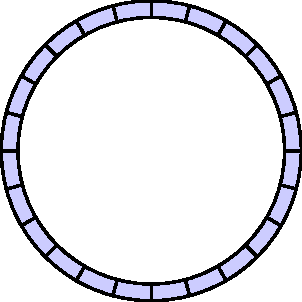
\includegraphics[width=.3\textwidth]{fig_circularList.pdf}
	  \caption{Condição de contorno periódica em um reticulado unidimensional formando um anel.}
	  \label{fig:anel}
	\end{figure}

	\begin{figure}[h!]
	  \centering
  	  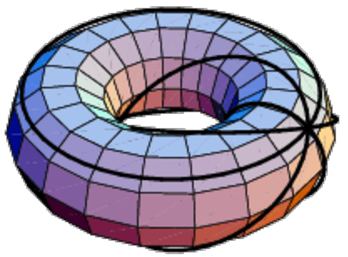
\includegraphics{fig_toro.pdf}
	  \caption{Condição de contorno periódica em um reticulado bidimensional formando um toroide.}
	  \label{fig:toro}
	\end{figure}

%Estados; regras locais; e raio
As células de um autômato celular podem apresentar $k$ estados. O valor desses estados é representado por valores inteiros no intervalo $[0, k-1]$, ou por cores. O estado de uma célula pode ser modificado pelas funções locais, que determinam o novo valor de uma célula baseado em seu estado atual e nos estados das células adjacentes. Para que as funções locais atualizem os valores de uma célula, é necessário que um raio $r$ seja definido. Esse raio $r$, por meio da fórmula $2r + 1$, representa o tamanho da vizinhança serão analisadas pelas funções locais. Para $r =0{,}5$, por exemplo, a vizinhança análisada terá duas células.

Além do raio, é preciso determinar o formato de vizinhança que será utilizada nos parâmetros da função local. Duas vizinhanças bem comuns em ACs bidimensionais são as vizinhanças de von Neumann \cite{weisstein2015b} e Moore \cite{weisstein2015c}. Na Figura \ref{fig:vVonNeumann} e na Figura \ref{fig:vMoore} são apresentadas, para raios de 0 a 3, as vizinhanças de von Neumann e Moore, respectivamente. No caso dos ACs unidimensionais, as vizinhanças são definidas apenas pelo raio $r$ e ele descreve quantas células à esquerda e direita da célula atual serão consideradas pela função local.

	\begin{figure}[h!]
	  \centering
	  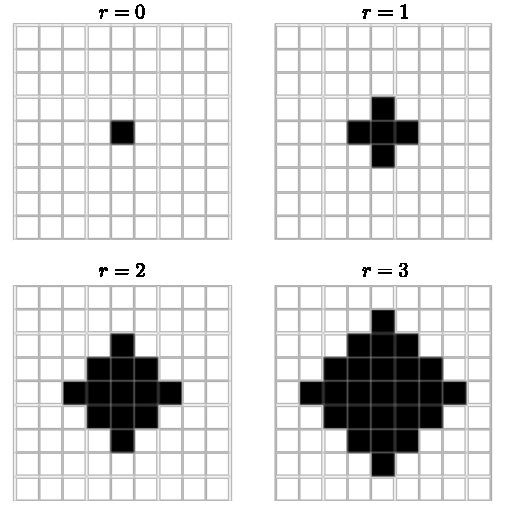
\includegraphics[width=0.45\textwidth]{fig_vVonNeumann.pdf}
	  \caption{Vizinhança de von Neumann com raio $r$ igual a 0, 1, 2 e 3. Essa foi a vizinhança utilizada nos primeiros trabalhos de von Neumann \cite{weisstein2015b}.}
	  \label{fig:vVonNeumann}
	\end{figure}

	\begin{figure}[h!]
	  \centering
  	  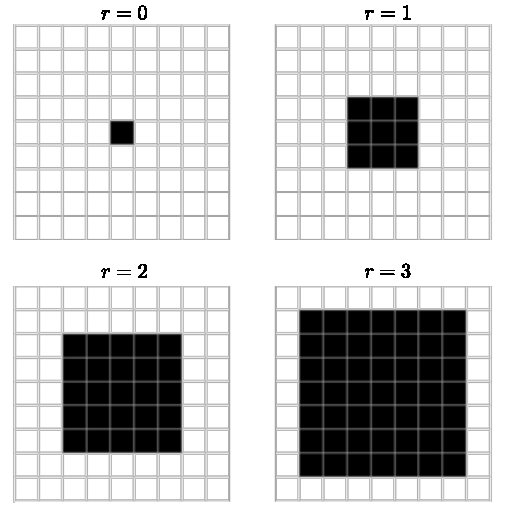
\includegraphics[width=0.45\textwidth]{fig_vMoore.pdf}
	  \caption{Vizinhança de Moore com raio $r$ igual a 0, 1, 2 e 3. Essa é a vizinhança utilizada no Jogo da Vida \cite{weisstein2015c}.}
	  \label{fig:vMoore}
	\end{figure}

%Famílias de autômatos Celulares; e Autômatos Celulares Elementares.
Uma família de autômatos celulares é definida pelo raio e pelo número de estados. Autômatos celulares unidimensionais de $r=1$ e $k=2$ são conhecidos como a família dos autômatos celulares elementares.

Todo AC é regido por um conjunto de regras locais que determinam como ficarão as configurações no próximo passo de tempo de acordo com as configurações de vizinhança recebidas. Existem diversas maneiras de representar essas regras locais, sendo que a mais comum são as tabelas de transições. A tabela de transições é uma tupla em que os elementos são todas as possíveis configurações de estado das vizinhanças de uma célula, acrescidos de um estado que representa a transição que ocorrerá. O primeiro item da tupla apresenta uma vizinhança formada por todas as células no estado $k – 1$, e o último item apresenta uma vizinhança formada apenas por estados $0$, sendo essa a ordenação lexicográfica de Wolfram. Cada regra também apresenta um número de identificação obtido ao se converter o resultado das transições de estados das tabelas para decimal. A Eq. \eqref{eq:nupla} representa a tupla da regra 30.
	\begin{equation}
	\begin{split}
	(((1,1,1),0),((1,1,0),0),((1,0,1),0),((1,0,0),1),\\
	((0,1,1),1),((0,1,0),1),((0,0,1),1),((0,0,0),0))
	\label{eq:nupla}
	\end{split}
	\end{equation}

Uma outra forma de representar uma tabela de transições é a forma icônica. Na forma icônica o bit $1$ é representado por um ícone na cor preta, e o bit $0$ por um ícone na cor branca. Cada uma das transições de estados é representada por um conjunto de ícones que simbolizam a vizinhança na parte superior, e o estado resultante após a transição, na parte inferior. A Figura \ref{fig:repIconicaR30} ilustra a representação icônica da regra 30.
	\begin{figure}[h!]
	  \centering
	  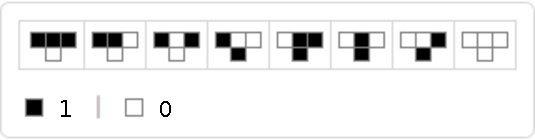
\includegraphics[width=0.45\textwidth]{fig_repIconicaR30.pdf}
	  \caption{Representação icônica da regra 30.}
	  \label{fig:repIconicaR30}
	\end{figure}

Além dessas formas de representação, ainda existe a forma $k$-ária em que, sabendo-se o valor atribuído para $k$ e $r$, elimina-se a representação das vizinhanças e deixa-se apenas as representações resultantes. Na Eq. \eqref{eq:karia} é possível ver a representação $k$-ária da regra 30. %TODO pois... explicar
	\begin{equation}
	(0,0,0,1,1,1,1,0)
	\label{eq:karia}
	\end{equation}

O número de regras de um espaço é dado pela Eq. \eqref{eq:tamFamilia}:%TODO explicar melhor
	\begin{equation}
	k^{k^{2r+1}}
	\label{eq:tamFamilia}
	\end{equation}

No espaço elementar há $2^{2^{3}} = 256$ regras. Aumentando o raio $r=2$, obtemos uma família de $2^{2^{5}} = 4.294.967.296$ regras. Para $k=3$ e $r=1$, obtém-se um espaço de ACs com $3^{3^{3}} = 7.625.597.484.987$ regras. Logo, é fácil perceber que qualquer modificação nas variáveis $k$ e $r$ geram famílias com número de regras muito grande. %TODO >>>>>>>>>>>>>>>>> Citar Algoritmos genéticos 
Famílias grandes de ACs representam um desafio na hora de encontrar ACs com propriedades específicas, já que procurar regras através de força bruta em um espaço muito grande se torna uma tarefa extremamente improdutiva. %TODO <<<<<<<<<<<<<<<<< Citar Algoritmos genéticos

Para contornar esse problema, é comum utilizar algumas propriedades estáticas para restringir as regras do espaço no qual serão feitas as buscas, no entanto,  faz-se necessário uma forma de representar essas propriedades e até mesmo aplicar operações como intersecção e diferença entre elas. Nesse ponto que os \textit{templates} apresentam-se de uma forma interessante e útil para representar conjuntos de regras com determinada propriedade. Templates de ACs são uma generalização das tabelas de transições que permitem representar espaços inteiros de ACs \cite{Verardo2014}. No Capítulo \ref{sec:templates} os templates serão explicados em mais detalhes e a no Capítulo \ref{sec:propriedadeEstaticasDef} são explicados algumas propriedades estáticas que podem ser representadas por templates. %Explicar porque o raio 3. vide p. 10